\input{"/users/l-wild/fjw/tex/preamble-master"}

\begin{document}
\title{Business Cycles and Productivity Shocks:\\ Are business cycles mostly the result of productivity shocks, or do shocks in nominal variables matter
too?}\author{Frederick Wild}\maketitle

\section{The Problem}


\textit{An important question from the “real business cycle” (RBC) literature (now superseded by/incorporated into the DSGE literature): are business cycles mainly
the result of permanent shocks to productivity? \cite{king_stochastic_1987} (KPSW) work with quarterly data from the US covering the period 1947-1988. The paper
starts with a review of the implications of balanced growth in the basic neoclassical growth model when combined with productivity shocks. In this model, per capita
consumption, investment and output (C, I and Y) all grow at the same rate. Add in a productivity shock and the expected long-run growth path changes. The upshot of
this is that the logs of C, I and Y should share a common stochastic trend, i.e., that they should be cointegrated. The question KPSW ask is: are business cycles
mostly the result of productivity shocks, or do shocks in nominal variables matter too? Your task in this project is to carry out a similar exercise for a country of
your choice. The techniques used in this project involve topics and techniques that are not covered in Economics 1 and Econometrics 2 (cointegration, VECMs, DOLS,
Johansen’s procedure, structural breaks, etc.), and therefore this topic should be taken up only by groups who either are willing to read up and master their
techniques on their own or who already have some expertise in them.}

\section{Theoretical Literature}

\subsection{Background on RBC}

\begin{enumerate}
  \item ``The central idea of the theory is that business cycles are “real” in that
they do not represent a failure of markets to clear but rather reflect the possibly most
efficient operations of the economy, given the structure of the economy and the
rationality of the economic agents.'' (\cite[p.8]{deng_real_2009})
\item s
\end{enumerate}


\subsection{VARs}

Chapters 16 and 17 of \cite{hansen_econometrics_2016} will be pretty useful here.


\subsection{Cointegration}

\subsection{VECMs}

\subsection{DOLS}

\subsection{Johansen's Procedure}

\subsection{Structural Breaks}





\section{Previous Empirical Work}

\subsection{KPSW}

\cite[p.11]{king_stochastic_1987} set up ``a general factor model representation of an $n$-dimensional vector $X_t$, where the common factors are random walks'':

\begin{align}
  X_t & = \gamma + Ar_t + D(L)\eps_t \\
  r_t & =  \mu + r_{t-1} +\eta_t
\end{align}

where $\gamma$ is a $n$ by 1 vector of constants, $r_t$ is a $k$ by 1 vector of random walks with drift $\mu$ and innovations $\eta_t$ (where $k\leq n$), $L$ is the
lag operator, $D(L)$ is a $n$ by $n$ matrix of lag polynomials, and $\eps_t$ a $n$ by 1 vector of serially uncorrelated, mean zero transitory innovations with
covariance matrix $\Sigma$.



\section{Our Project}

\subsection{Establish motivation}

The first thing we do should be to establish the feature of the economy we're looking at. I think a good first step would be to
plot log deviations of consumption, investment, and GNP to show

\begin{enumerate}
  \item Cyclical variability. All variables show certain volatility over time with
  repetitive patterns, though magnitudes of the fluctuations are different.
  \item Correlation. The co-movements of output and other variables are quite
  evident except for the capital stock. Although with different levels, all
  variables are pro-cyclical, while capital stock seems acyclical.
  \item Persistence. If we take any point in the series above the trend, the
  probability that the next period is still above-trend is very high. However,
  this persistence appears to wear out over time.
\end{enumerate}

All of above from \cite[p.9]{deng_real_2009}. Using the \href{http://www.rug.nl/ggdc/productivity/pwt/}{Penn World Table} data on national accounts, we get Figure
\ref{fig:deviations}.

\begin{figure}[!htpb]
  \centering
  \caption{Log Deviations of GDP, Consumption and Investment for Great Britain, 1950-2014}
  \label{fig:deviations}
  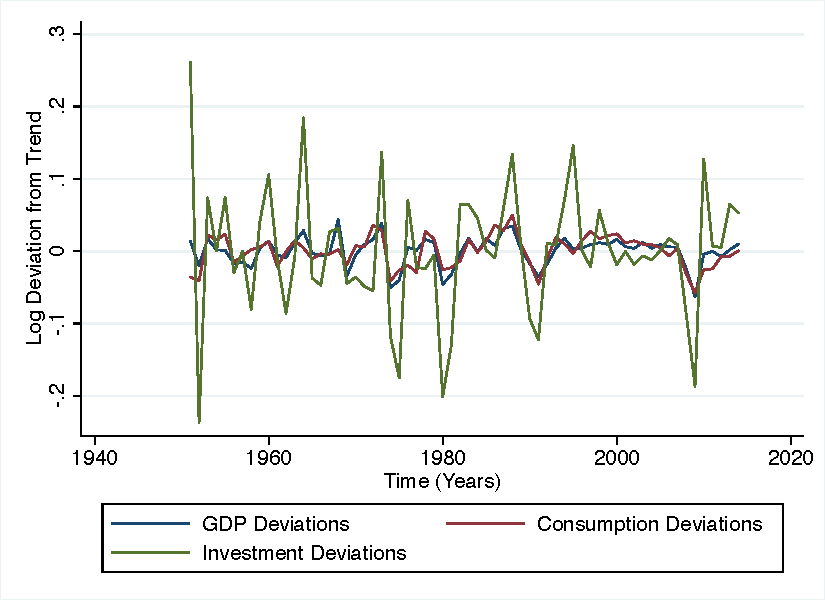
\includegraphics[width=\textwidth]{/Users/l-wild/FJW/project/graphics/dev_time_na.pdf}
\end{figure}


which all ends up looking quite nice. This comes from an OLS regression of the log changes in each of the variables on time and a constant, then using these
predicted values to form the trend. Finally, subtract the log changes in the variables from their predicted time value. I also plot the trend for our
variables and the deviations from trend in Figure \ref{fig:deviations2}.

\begin{figure}[!htpb]
  \centering
  \caption{Trends and Deviations in GDP, Consumption and Investment for Great Britain, 1950-2014}
  \label{fig:deviations2}
  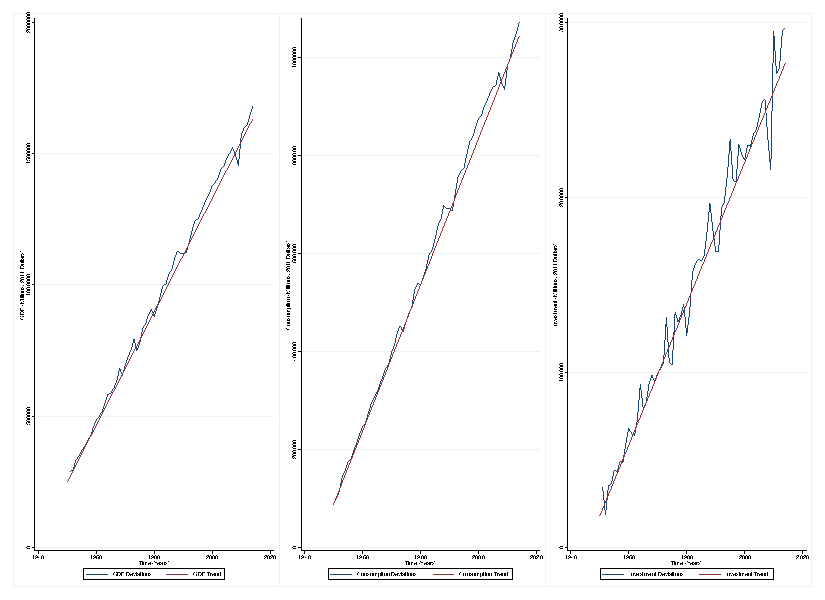
\includegraphics[width=\textwidth]{/Users/l-wild/FJW/project/graphics/trend_time_na.pdf}
\end{figure}


\subsection{Data}

I used UK above, but plenty of other countries to choose from. We use data at constant 2011 prices (current-year price also available)

\subsection{Model}



\subsection{Method}

\subsection{Results}





\printbibliography




\end{document}
